% Setting up the document class and necessary packages
\documentclass[a4paper,12pt]{article}
\usepackage[utf8]{inputenc}
\usepackage[T1]{fontenc}
\usepackage{lmodern} % Latin Modern font for better compatibility
\usepackage{geometry}
\geometry{margin=1in}
\usepackage{graphicx} % For including figures
\usepackage{caption} % For figure captions
\usepackage{booktabs} % For professional tables
\usepackage{enumitem} % For better list formatting
\usepackage{amsmath} % For mathematical formatting if needed
\usepackage{xcolor} % For colored text
\usepackage{hyperref} % For hyperlinks
\usepackage{parskip} % For paragraph spacing
\usepackage{float} % For better figure placement
\setlength{\parskip}{0.5em}
\setlength{\parindent}{0em}

% Setting up font to Noto Serif for consistency
% \usepackage{noto} % Commented out - may not be available on all systems

% Title page setup
\title{Sentiment Analysis Report: Electricity Issues in Rwanda}
\author{}
\date{July 13, 2025}

\begin{document}
	
	% Creating the title page
	\maketitle
	\begin{center}
		\vspace{0.5cm}
		\textbf{Prepared for Assignment on Sentiment Analysis and Web Scraping}
	\end{center}
	
	\newpage
	
	% Abstract
	\begin{abstract}
		This report presents a sentiment analysis of social media posts related to electricity services in Rwanda, focusing on interactions with the Rwanda Energy Group (@reg\_rwanda). Using a keyword-based approach with fuzzy matching, we analyzed 148 user posts and 25 @reg\_rwanda responses, identifying sentiment distributions, common locations, and prevalent issues. The analysis reveals significant public dissatisfaction, with 72.3\% of user posts expressing negative sentiment, particularly in Rubavu, and frequent mentions of electricity (``umuriro''). Visualizations, including pie charts, bar charts, and a word cloud, support the findings. The report concludes with recommendations for addressing public concerns and improving service delivery.
	\end{abstract}
	
	% Section: Introduction
	\section{Introduction}
	Electricity reliability is a cornerstone of Rwanda's development goals, impacting households, businesses, and economic growth. As Rwanda pursues universal electricity access, public sentiment on social media provides valuable insights into service challenges and user experiences. This report analyzes posts from X related to @reg\_rwanda, the X handle for the Rwanda Energy Group, to assess public sentiment, identify key issues (e.g., outages, cashpower), and highlight affected regions. The analysis leverages keyword-based sentiment classification and fuzzy matching to account for linguistic variations in Kinyarwanda and English, offering a comprehensive view of public perceptions.
	
	% Section: Methodology
	\section{Methodology}
	
	\subsection{Data Source}
	The dataset used in this study was obtained from a file named \texttt{x.csv}, which contains social media posts scraped from X (formerly Twitter). Data collection was performed using Instant Data Scraper, an automated web scraping tool that extracts structured information from web pages and exports it into CSV format. The dataset includes user-generated posts along with replies from the official account @reg\_rwanda. For analysis purposes, two text fields—\texttt{css-1jxf684 5} and \texttt{css-1jxf684 4}—were merged into a single field named \texttt{raw\_text}, which consolidates the relevant content from each post.
	
	\subsection{Data Preprocessing}
	The data preprocessing involved several key steps:
	\begin{itemize}
		\item \textbf{Cleaning}: Removed duplicates based on username, text, and URL. Filtered out irrelevant posts containing phrases like ``show more replies'' or ``who to follow'' using regular expressions.
		\item \textbf{Text Normalization}: Converted text to lowercase, removed special characters, and normalized whitespace.
		\item \textbf{Filtering}: Excluded posts with fewer than 7 words or lacking relevant keywords (sentiment or location-related).
	\end{itemize}
	
	\subsection{Sentiment Classification}
	Sentiment was classified as positive, negative, or neutral using predefined keyword lists tailored to the Rwandan context:
	\begin{itemize}
		\item \textbf{Positive Keywords}: e.g., ``murakoze'' (thank you), ``power is back'', ``resolved''.
		\item \textbf{Negative Keywords}: e.g., ``ikibazo'' (problem), ``outage'', ``no power''.
		\item \textbf{Neutral Keywords}: e.g., ``ese'' (question), ``when'', location names.
	\end{itemize}
	
	Fuzzy matching (via the \texttt{fuzzywuzzy} library) with a 75\% similarity threshold was used to handle spelling variations. @reg\_rwanda responses were classified with additional logic to avoid misclassifying polite responses as positive. Posts were labeled neutral if only location names were matched or no sentiment keywords were found.
	
	\subsection{Analysis Approach}
	The analysis methodology included:
	\begin{itemize}
		\item Separated user posts (N=148) and @reg\_rwanda responses (N=25) for distinct analysis.
		\item Counted sentiment distributions and calculated percentages.
		\item Identified mentions of locations (e.g., Rubavu, Huye) and issues (e.g., umuriro, cashpower) using regular expressions.
		\item Generated visualizations using Plotly and Matplotlib, saved as PNG files.
	\end{itemize}
	
	% Section: Results
	\section{Results}
	
	\subsection{Overall Sentiment Distribution}
	The analysis processed 148 user posts and 25 @reg\_rwanda responses, revealing significant patterns in public sentiment toward electricity services.
	
	\subsubsection{User Posts Sentiment}
	The sentiment distribution among user posts shows people's negative sentiment:
	\begin{itemize}
		\item Negative: 107 posts (72.3\%)
		\item Neutral: 27 posts (18.2\%)
		\item Positive: 14 posts (9.5\%)
	\end{itemize}
	
	\begin{figure}[H]
		\centering
		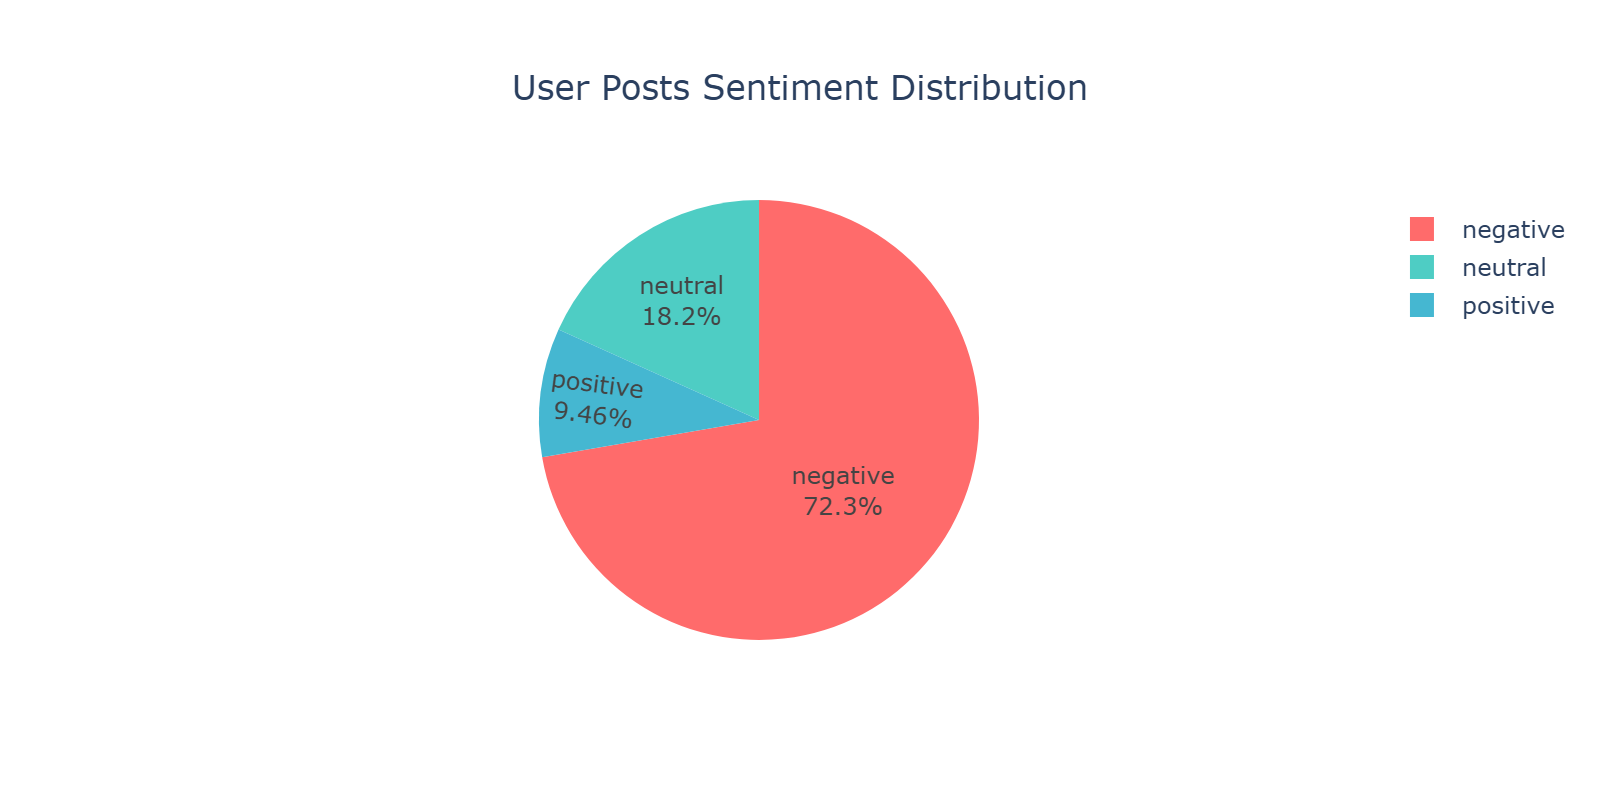
\includegraphics[width=0.7\textwidth]{../results/user_sentiment_distribution.png}
		\caption{User Sentiment Distribution - The pie chart clearly shows the dominance of negative sentiment (72.3\%) among user posts, indicating widespread dissatisfaction with electricity services.}
		\label{fig:user_sentiment}
	\end{figure}
	
	\subsubsection{@reg\_rwanda Response Sentiment}
	The official responses from @reg\_rwanda show a more balanced sentiment distribution:
	\begin{itemize}
		\item Negative: 9 posts (36.0\%)
		\item Positive: 9 posts (36.0\%)
		\item Neutral: 7 posts (28.0\%)
	\end{itemize}
	
	\begin{figure}[H]
		\centering
		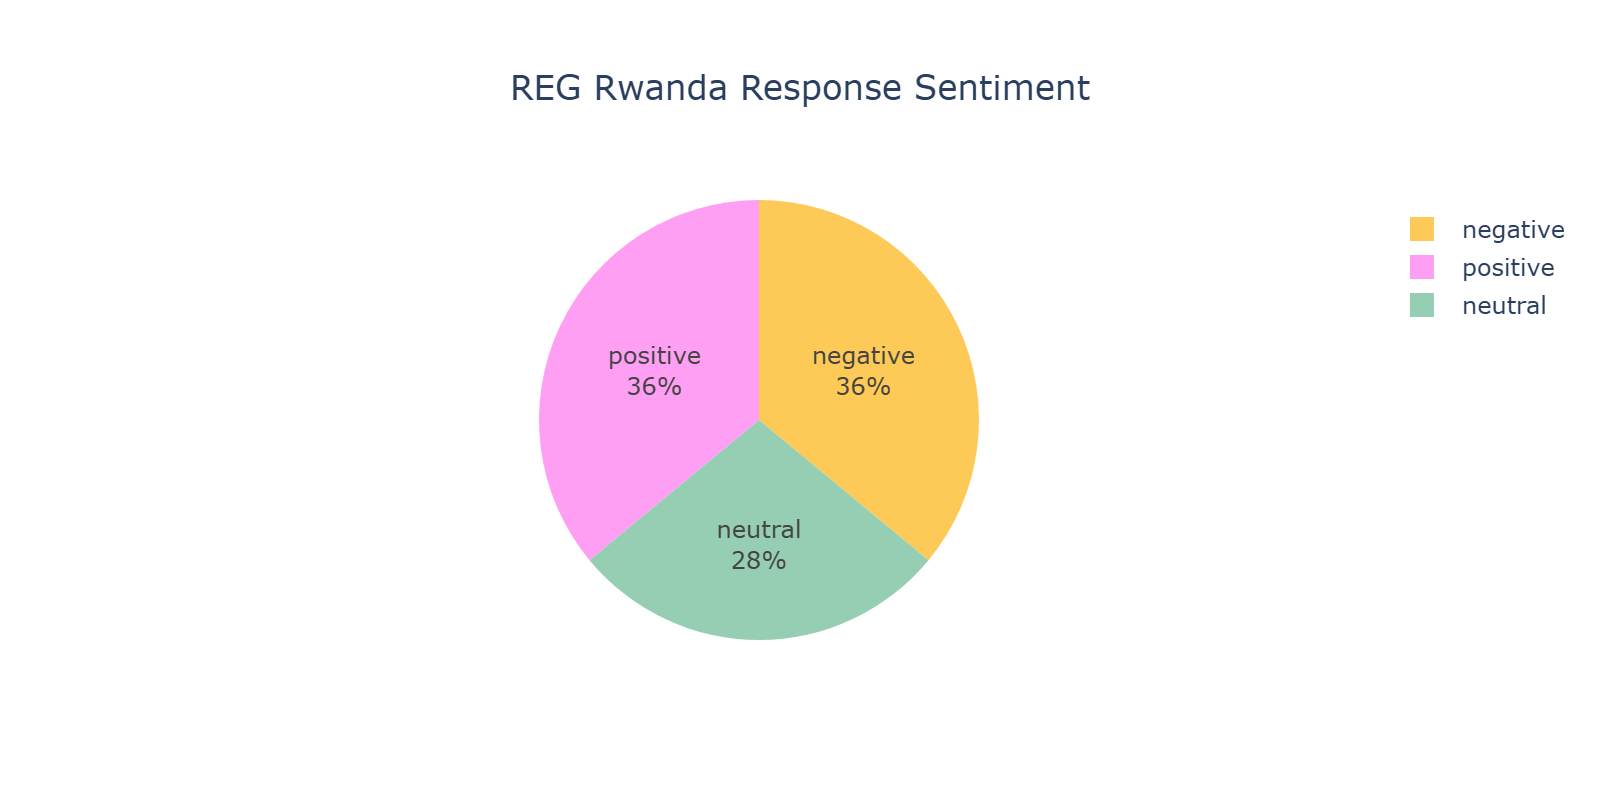
\includegraphics[width=0.7\textwidth]{../results/reg_sentiment_distribution.png}
		\caption{@reg\_rwanda Sentiment Distribution - Official responses show balanced sentiment with equal proportions of positive and negative responses (36\% each).}
		\label{fig:reg_sentiment}
	\end{figure}
	
	\subsubsection{Sentiment Comparison}
	A direct comparison between user posts and official responses reveals the stark contrast in sentiment patterns.
	
	\begin{figure}[H]
		\centering
		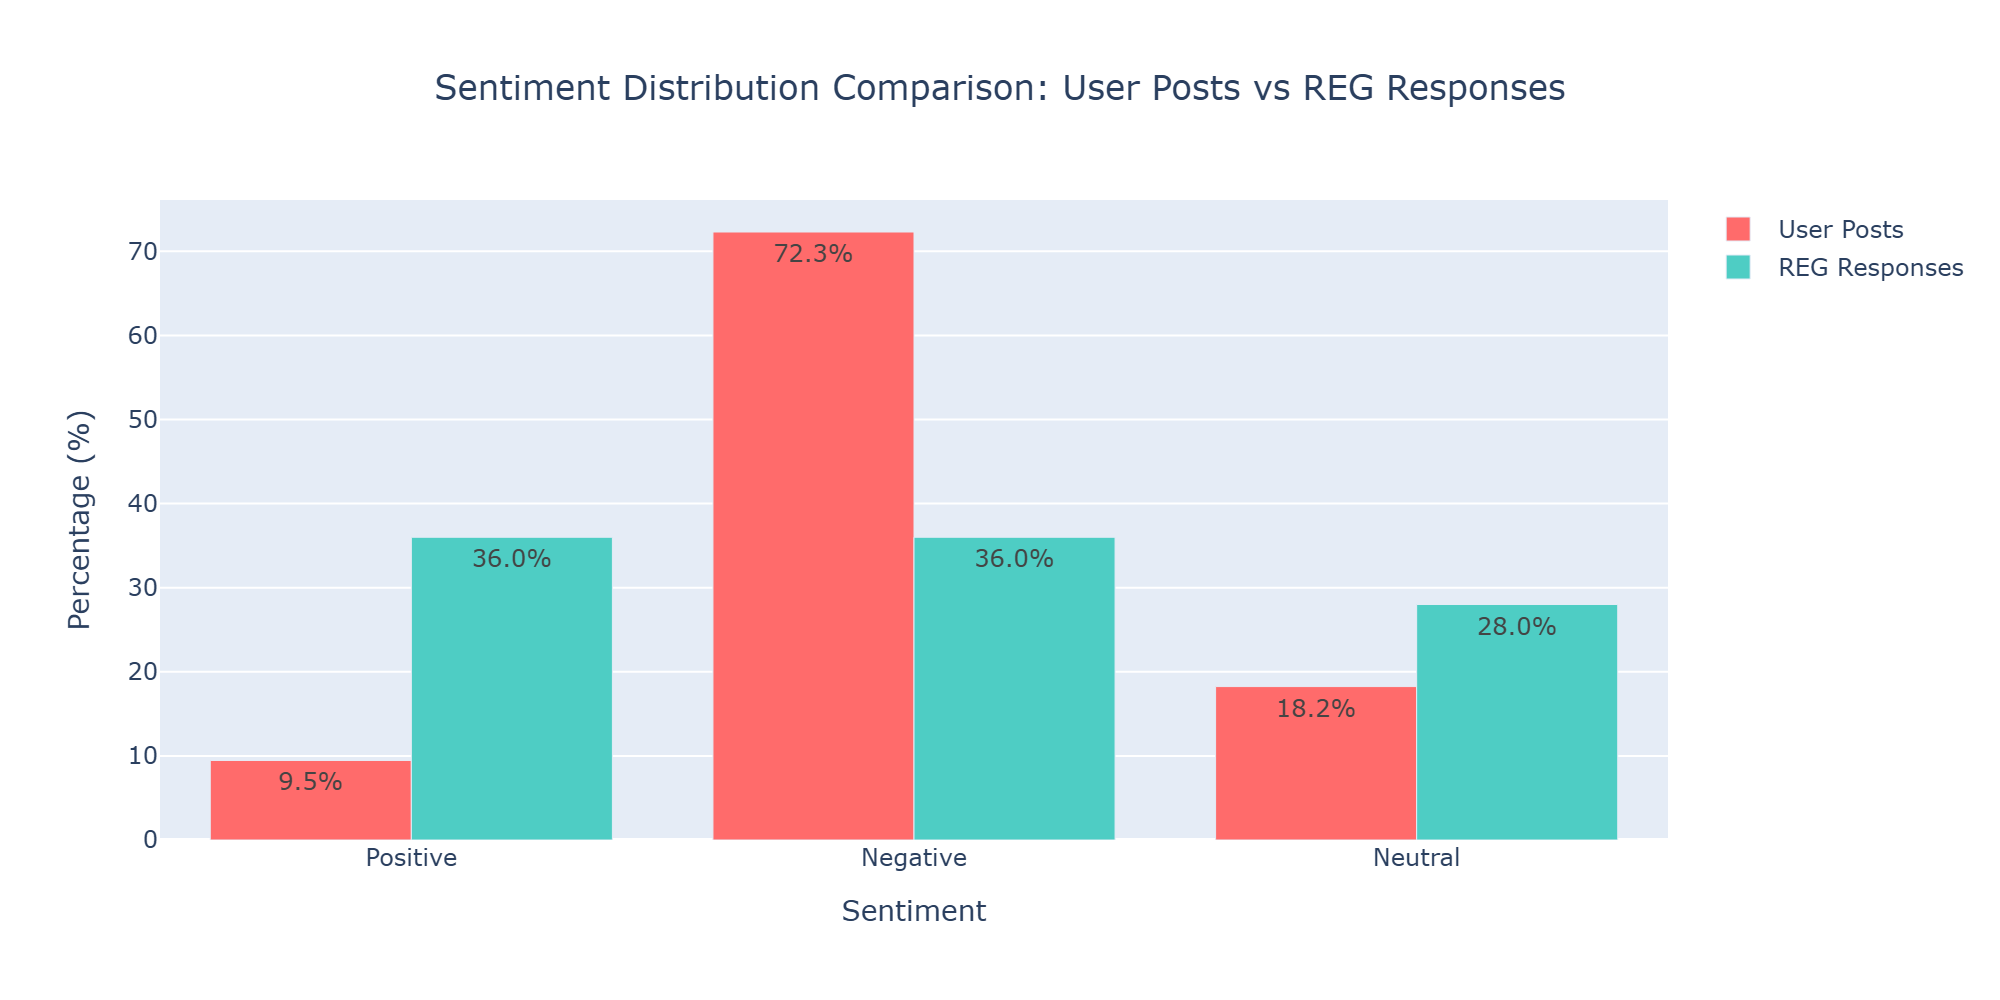
\includegraphics[width=0.8\textwidth]{../results/sentiment_comparison.png}
		\caption{Sentiment Comparison Between Users and @reg\_rwanda - This grouped bar chart highlights the significant difference in sentiment patterns, with users showing predominantly negative sentiment while official responses are more balanced.}
		\label{fig:sentiment_comparison}
	\end{figure}
	
	\subsection{Geographic Analysis}
	
	\subsubsection{Most Affected Locations}
	The analysis identified specific locations with high complaint frequencies:
	\begin{itemize}
		\item Rubavu: 16 mentions (highest)
		\item Huye: 7 mentions
		\item Kicukiro: 6 mentions
		\item Kimironko: 6 mentions
		\item Bugesera: 5 mentions
	\end{itemize}
	
	Other locations such as Nyarugenge and Musanze had fewer mentions but still represent areas of concern.
	
	\begin{figure}[H]
		\centering
		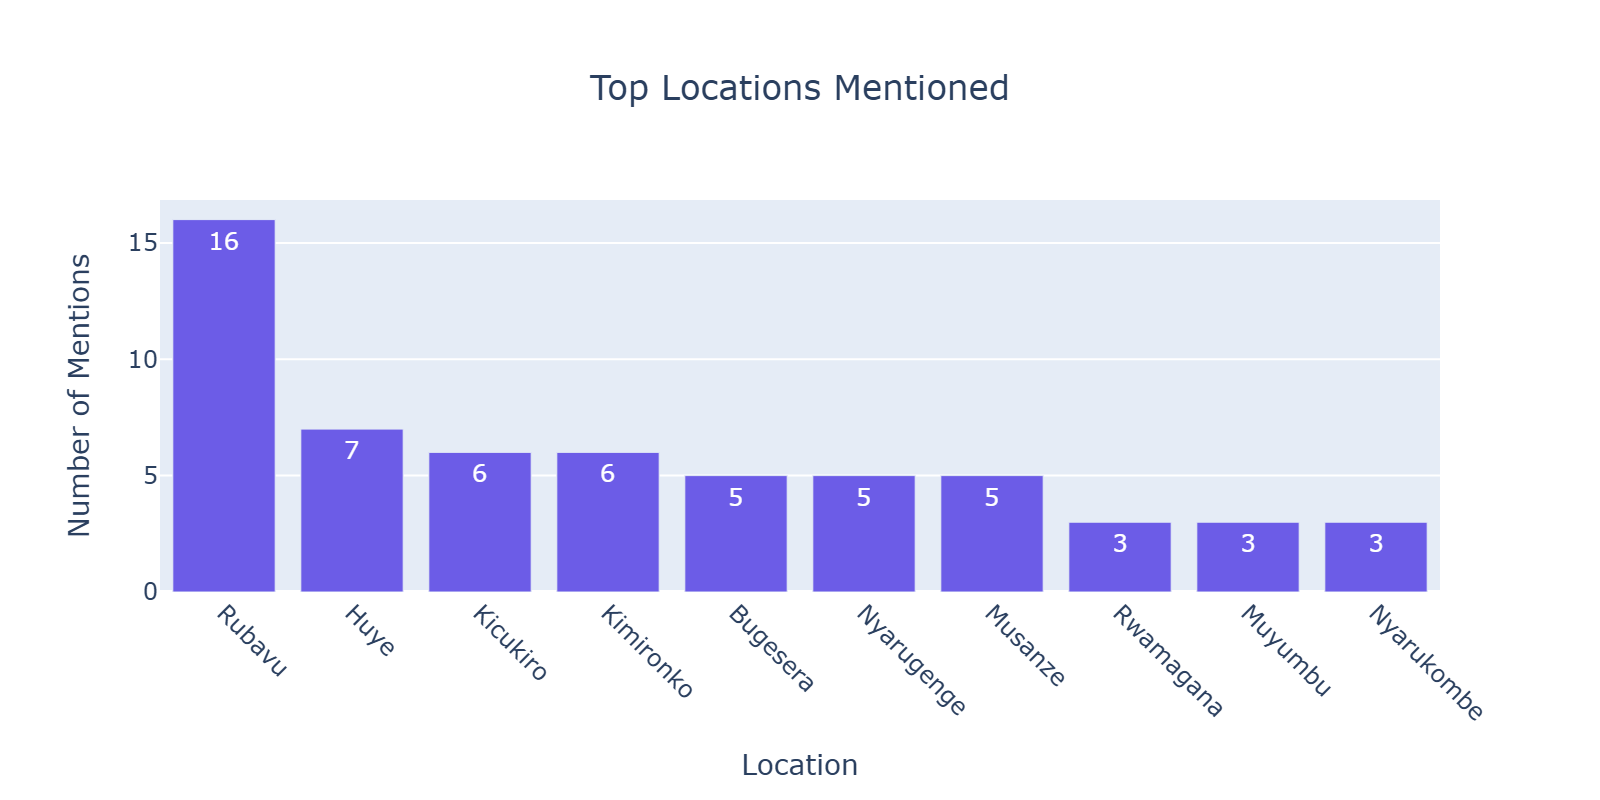
\includegraphics[width=0.8\textwidth]{../results/top_locations.png}
		\caption{Top Locations Mentioned in User Posts - Rubavu stands out as the location with the highest number of electricity-related complaints, suggesting regional infrastructure challenges.}
		\label{fig:top_locations}
	\end{figure}
	
	\subsubsection{Sentiment by Location}
	The geographic distribution of sentiment reveals location-specific patterns in user satisfaction.
	
	\begin{figure}[H]
		\centering
		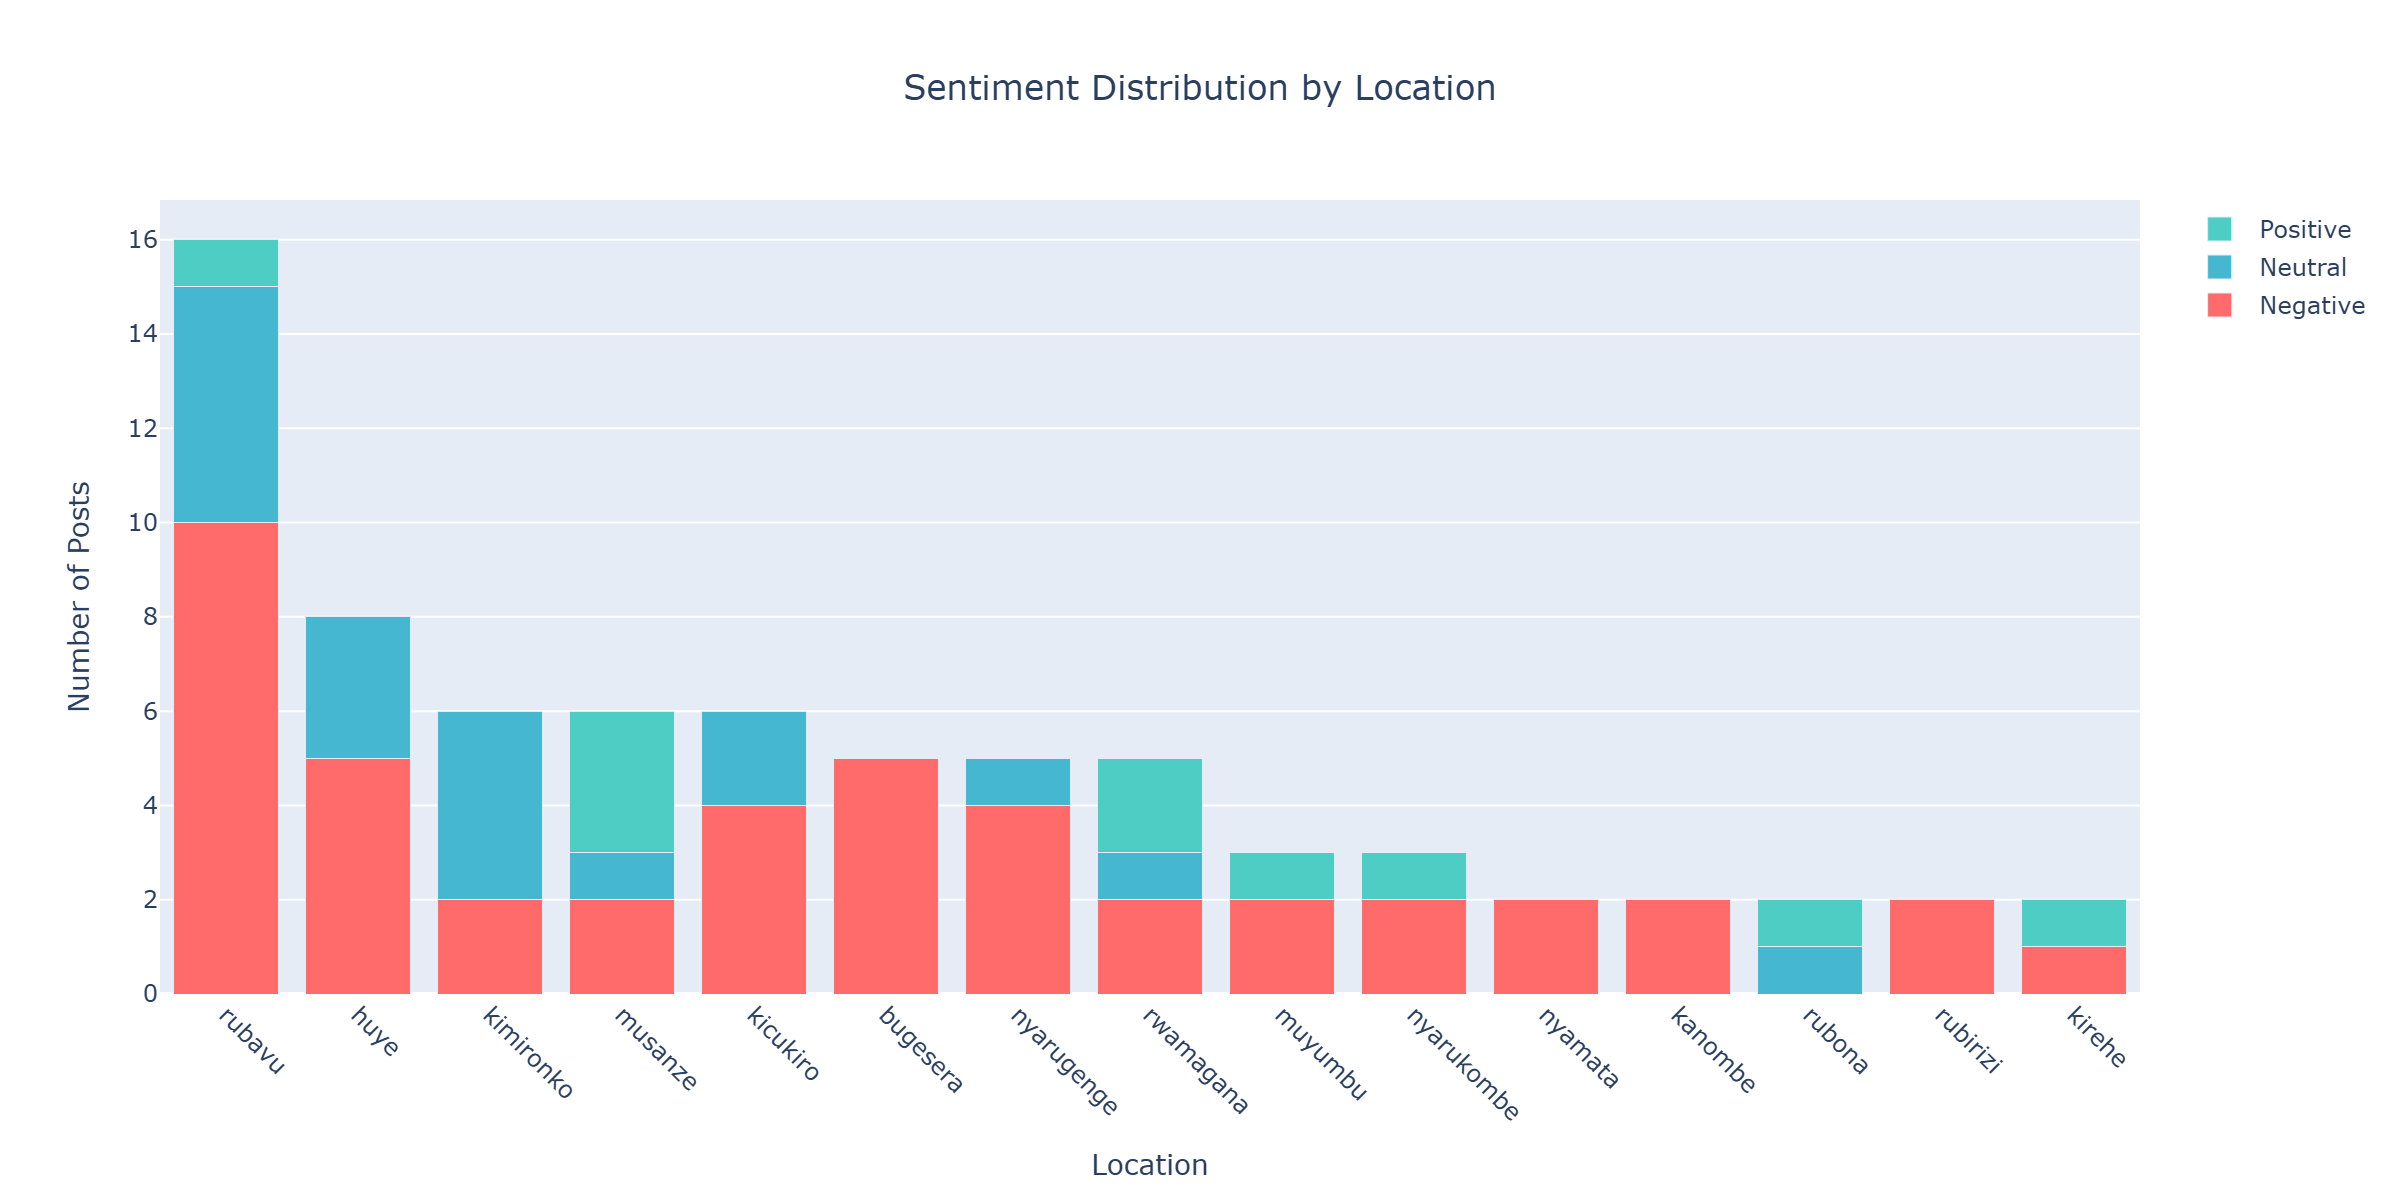
\includegraphics[width=0.9\textwidth]{../results/sentiment_by_location.png}
		\caption{Sentiment Distribution Across Top 15 Locations - This stacked bar chart shows how sentiment varies across different locations, with most areas showing predominantly negative sentiment.}
		\label{fig:sentiment_location}
	\end{figure}
	
	\subsection{Issue Analysis}
	
	\subsubsection{Most Common Issues}
	The frequency analysis of reported issues reveals:
	\begin{itemize}
		\item Umuriro (electricity): 62 mentions (most frequent)
		\item Ikibazo (problem): 25 mentions
		\item Cashpower: 8 mentions
		\item Outage: 4 mentions
		\item Token: 3 mentions
	\end{itemize}
	
	\begin{figure}[H]
		\centering
		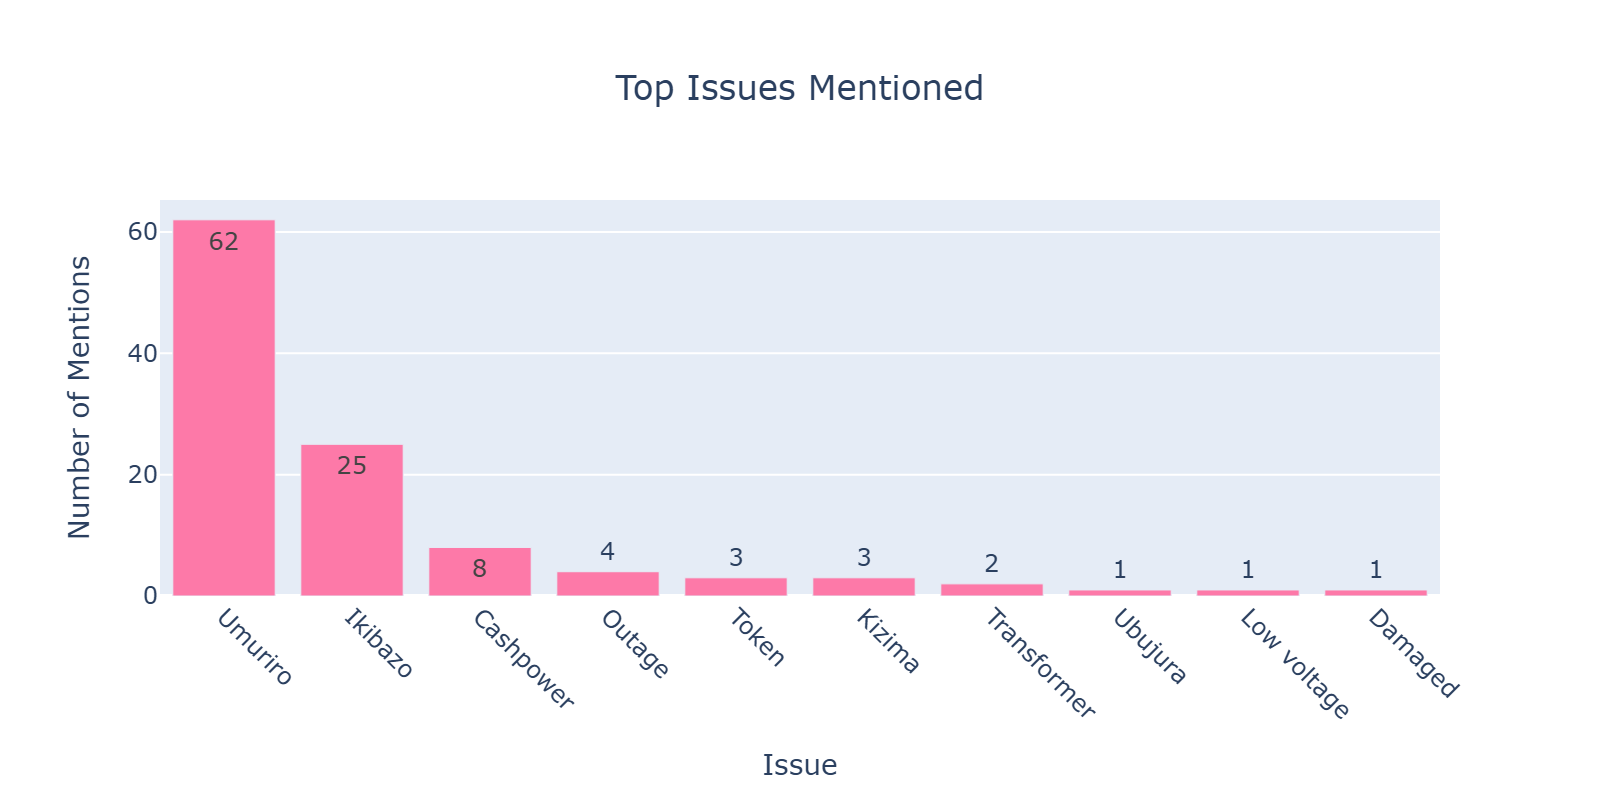
\includegraphics[width=0.8\textwidth]{../results/top_issues.png}
		\caption{Top Issues Mentioned in User Posts - "Umuriro" (electricity) dominates the issues mentioned, being referenced 62 times, indicating it as the primary concern among users.}
		\label{fig:top_issues}
	\end{figure}
	
	\subsubsection{Negative Sentiment Keywords}
	A word cloud visualization of negative sentiment posts provides insights into the most commonly used terms expressing dissatisfaction.
	
	\begin{figure}[H]
		\centering
		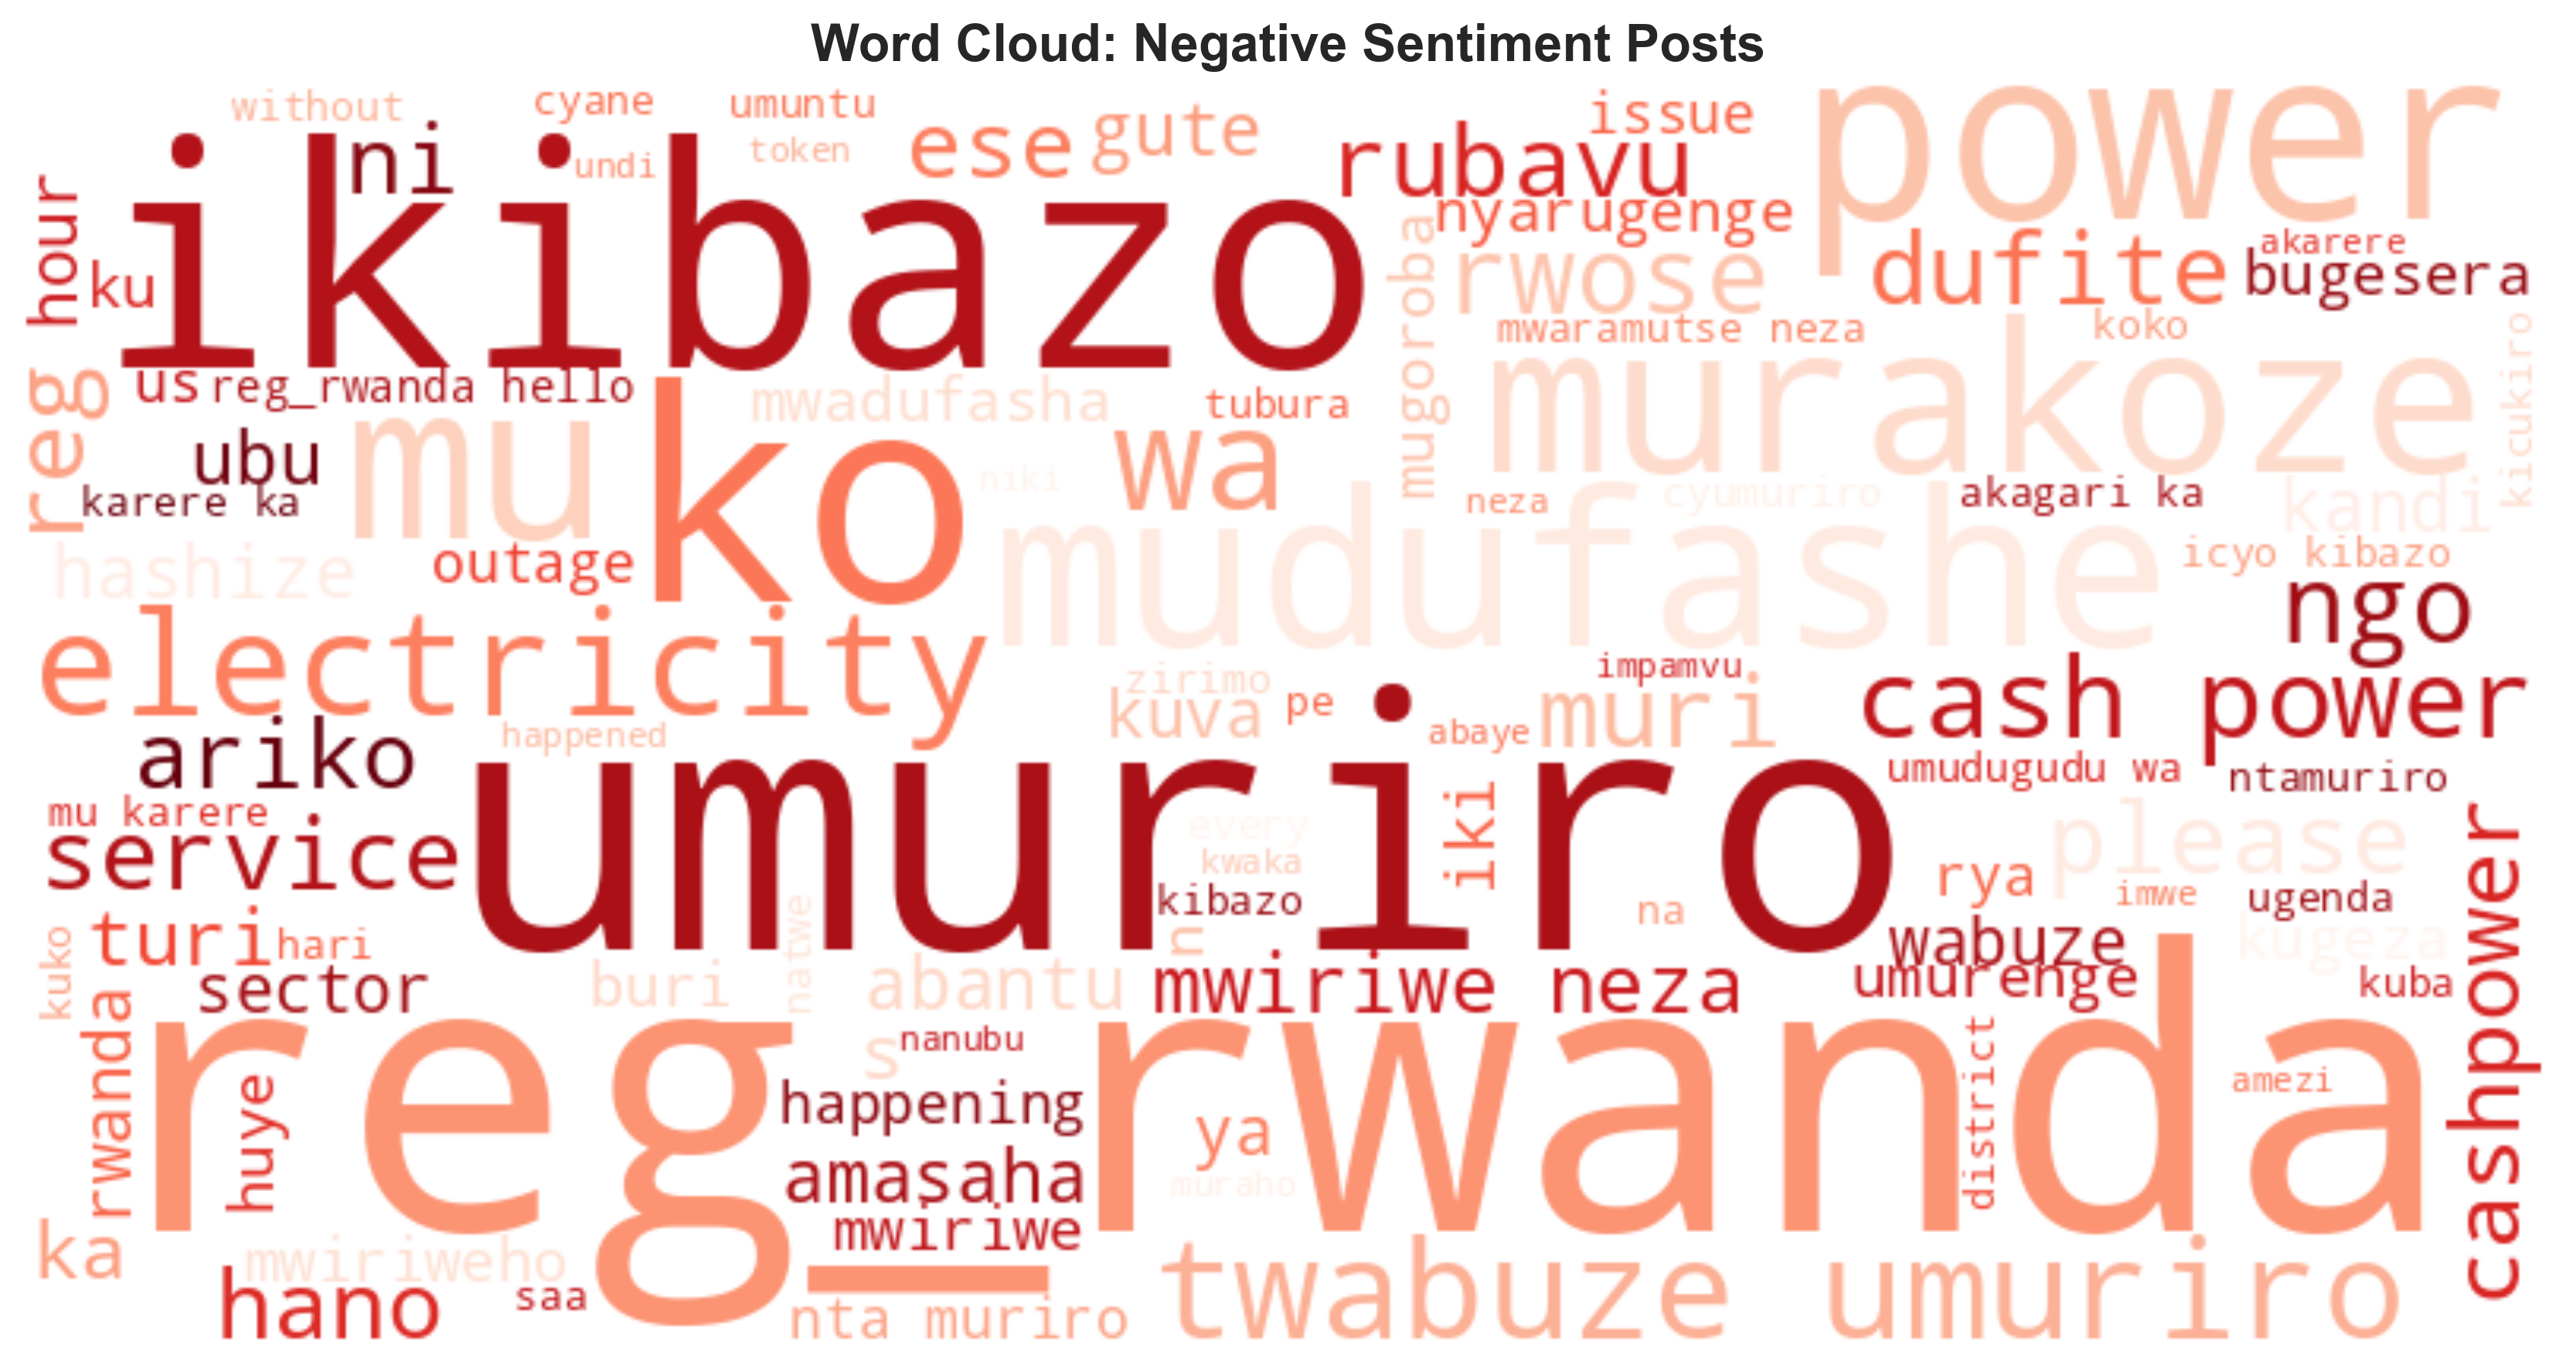
\includegraphics[width=0.8\textwidth]{../results/negative_wordcloud.png}
		\caption{Word Cloud of Negative Sentiment Posts - This visualization highlights the most frequently used terms in negative posts, with "umuriro" and "ikibazo" being prominently featured.}
		\label{fig:wordcloud}
	\end{figure}
	
	\subsection{Response Effectiveness Analysis}
	The effectiveness of @reg\_rwanda's engagement with user concerns was measured through response and resolution rates.
	
	\begin{figure}[H]
		\centering
		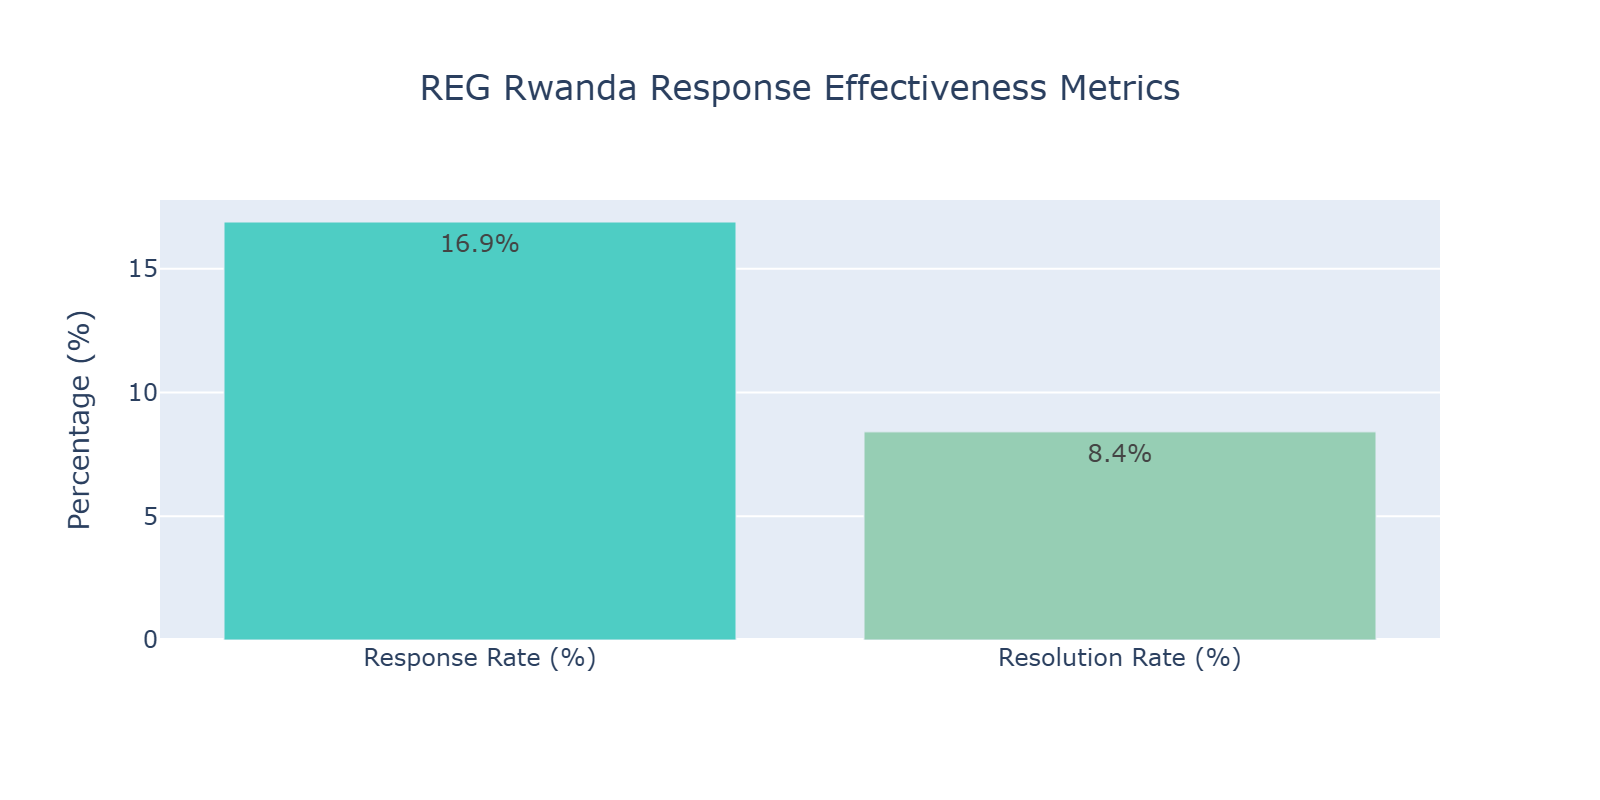
\includegraphics[width=0.8\textwidth]{../results/response_effectiveness.png}
		\caption{Response Effectiveness Metrics - The analysis shows a response rate of 16.9\% and resolution rate of 8.4\%, indicating limited effectiveness in addressing user concerns through social media engagement.}
		\label{fig:effectiveness}
	\end{figure}
	
	The low response rate (16.9\%) and even lower resolution rate (8.4\%) suggest that @reg\_rwanda's social media engagement strategy may need improvement to better address public concerns.
	
	\section{Key Findings}
	
	\subsection{Interesting Fact}
	The analysis reveals that 72.3\% of user posts express negative sentiment, with ``umuriro'' (electricity) mentioned 62 times, far exceeding other issues. This highlights widespread public frustration with power outages, particularly in Rubavu (16 mentions), suggesting regional disparities in electricity reliability that warrant targeted interventions.
	
	\subsection{Regional Disparities}
	Rubavu emerges as a particular hotspot for electricity-related complaints, with 16 mentions - more than double the next highest location (Huye with 7 mentions). This suggests specific infrastructure challenges in the Rubavu region that require focused attention.
	
	\subsection{Language Patterns}
	The predominant use of Kinyarwanda terms like ``umuriro'' and ``ikibazo'' in complaints indicates that users are more comfortable expressing their frustrations in their native language, which has implications for customer service approaches.
	
	\section{Conclusion}
	The sentiment analysis underscores significant public dissatisfaction with electricity services in Rwanda, with 72.3\% of 148 user posts classified as negative. Frequent mentions of ``umuriro'' and ``ikibazo'' indicate persistent issues with power supply and general problems. Rubavu emerges as a hotspot for complaints, likely due to infrastructure challenges. 
	
	@reg\_rwanda's responses show a balanced sentiment (36\% positive, 36\% negative, 28\% neutral), but the low resolution rate (8.4\%) suggests limited effectiveness in addressing user concerns. The visualizations provide clear insights into sentiment patterns, geographic distribution of issues, and the effectiveness of current response mechanisms.
	
	\section{References}
	\begin{itemize}
		\item Rwanda Energy Group. (2025). Official X Account (@reg\_rwanda). Retrieved from \url{https://x.com/reg_rwanda}.
		\item Instant Data Scraper. (2025). Automated Web Scraping Tool. Retrieved from \url{https://www.instantdatascraper.com/}.
		\item Plotly. (2025). Python Graphing Library. Retrieved from \url{https://plotly.com/python/}.
		\item Matplotlib. (2025). Python Visualization Library. Retrieved from \url{https://matplotlib.org/}.
		\item FuzzyWuzzy. (2025). Fuzzy String Matching in Python. Retrieved from \url{https://github.com/seatgeek/fuzzywuzzy}.
	\end{itemize}
	
\end{document}